% Options for packages loaded elsewhere
\PassOptionsToPackage{unicode}{hyperref}
\PassOptionsToPackage{hyphens}{url}
\PassOptionsToPackage{dvipsnames,svgnames,x11names}{xcolor}
%
\documentclass[
  letterpaper,
  DIV=11,
  numbers=noendperiod]{scrartcl}

\usepackage{amsmath,amssymb}
\usepackage{iftex}
\ifPDFTeX
  \usepackage[T1]{fontenc}
  \usepackage[utf8]{inputenc}
  \usepackage{textcomp} % provide euro and other symbols
\else % if luatex or xetex
  \usepackage{unicode-math}
  \defaultfontfeatures{Scale=MatchLowercase}
  \defaultfontfeatures[\rmfamily]{Ligatures=TeX,Scale=1}
\fi
\usepackage{lmodern}
\ifPDFTeX\else  
    % xetex/luatex font selection
\fi
% Use upquote if available, for straight quotes in verbatim environments
\IfFileExists{upquote.sty}{\usepackage{upquote}}{}
\IfFileExists{microtype.sty}{% use microtype if available
  \usepackage[]{microtype}
  \UseMicrotypeSet[protrusion]{basicmath} % disable protrusion for tt fonts
}{}
\makeatletter
\@ifundefined{KOMAClassName}{% if non-KOMA class
  \IfFileExists{parskip.sty}{%
    \usepackage{parskip}
  }{% else
    \setlength{\parindent}{0pt}
    \setlength{\parskip}{6pt plus 2pt minus 1pt}}
}{% if KOMA class
  \KOMAoptions{parskip=half}}
\makeatother
\usepackage{xcolor}
\setlength{\emergencystretch}{3em} % prevent overfull lines
\setcounter{secnumdepth}{5}
% Make \paragraph and \subparagraph free-standing
\ifx\paragraph\undefined\else
  \let\oldparagraph\paragraph
  \renewcommand{\paragraph}[1]{\oldparagraph{#1}\mbox{}}
\fi
\ifx\subparagraph\undefined\else
  \let\oldsubparagraph\subparagraph
  \renewcommand{\subparagraph}[1]{\oldsubparagraph{#1}\mbox{}}
\fi

\usepackage{color}
\usepackage{fancyvrb}
\newcommand{\VerbBar}{|}
\newcommand{\VERB}{\Verb[commandchars=\\\{\}]}
\DefineVerbatimEnvironment{Highlighting}{Verbatim}{commandchars=\\\{\}}
% Add ',fontsize=\small' for more characters per line
\usepackage{framed}
\definecolor{shadecolor}{RGB}{241,243,245}
\newenvironment{Shaded}{\begin{snugshade}}{\end{snugshade}}
\newcommand{\AlertTok}[1]{\textcolor[rgb]{0.68,0.00,0.00}{#1}}
\newcommand{\AnnotationTok}[1]{\textcolor[rgb]{0.37,0.37,0.37}{#1}}
\newcommand{\AttributeTok}[1]{\textcolor[rgb]{0.40,0.45,0.13}{#1}}
\newcommand{\BaseNTok}[1]{\textcolor[rgb]{0.68,0.00,0.00}{#1}}
\newcommand{\BuiltInTok}[1]{\textcolor[rgb]{0.00,0.23,0.31}{#1}}
\newcommand{\CharTok}[1]{\textcolor[rgb]{0.13,0.47,0.30}{#1}}
\newcommand{\CommentTok}[1]{\textcolor[rgb]{0.37,0.37,0.37}{#1}}
\newcommand{\CommentVarTok}[1]{\textcolor[rgb]{0.37,0.37,0.37}{\textit{#1}}}
\newcommand{\ConstantTok}[1]{\textcolor[rgb]{0.56,0.35,0.01}{#1}}
\newcommand{\ControlFlowTok}[1]{\textcolor[rgb]{0.00,0.23,0.31}{#1}}
\newcommand{\DataTypeTok}[1]{\textcolor[rgb]{0.68,0.00,0.00}{#1}}
\newcommand{\DecValTok}[1]{\textcolor[rgb]{0.68,0.00,0.00}{#1}}
\newcommand{\DocumentationTok}[1]{\textcolor[rgb]{0.37,0.37,0.37}{\textit{#1}}}
\newcommand{\ErrorTok}[1]{\textcolor[rgb]{0.68,0.00,0.00}{#1}}
\newcommand{\ExtensionTok}[1]{\textcolor[rgb]{0.00,0.23,0.31}{#1}}
\newcommand{\FloatTok}[1]{\textcolor[rgb]{0.68,0.00,0.00}{#1}}
\newcommand{\FunctionTok}[1]{\textcolor[rgb]{0.28,0.35,0.67}{#1}}
\newcommand{\ImportTok}[1]{\textcolor[rgb]{0.00,0.46,0.62}{#1}}
\newcommand{\InformationTok}[1]{\textcolor[rgb]{0.37,0.37,0.37}{#1}}
\newcommand{\KeywordTok}[1]{\textcolor[rgb]{0.00,0.23,0.31}{#1}}
\newcommand{\NormalTok}[1]{\textcolor[rgb]{0.00,0.23,0.31}{#1}}
\newcommand{\OperatorTok}[1]{\textcolor[rgb]{0.37,0.37,0.37}{#1}}
\newcommand{\OtherTok}[1]{\textcolor[rgb]{0.00,0.23,0.31}{#1}}
\newcommand{\PreprocessorTok}[1]{\textcolor[rgb]{0.68,0.00,0.00}{#1}}
\newcommand{\RegionMarkerTok}[1]{\textcolor[rgb]{0.00,0.23,0.31}{#1}}
\newcommand{\SpecialCharTok}[1]{\textcolor[rgb]{0.37,0.37,0.37}{#1}}
\newcommand{\SpecialStringTok}[1]{\textcolor[rgb]{0.13,0.47,0.30}{#1}}
\newcommand{\StringTok}[1]{\textcolor[rgb]{0.13,0.47,0.30}{#1}}
\newcommand{\VariableTok}[1]{\textcolor[rgb]{0.07,0.07,0.07}{#1}}
\newcommand{\VerbatimStringTok}[1]{\textcolor[rgb]{0.13,0.47,0.30}{#1}}
\newcommand{\WarningTok}[1]{\textcolor[rgb]{0.37,0.37,0.37}{\textit{#1}}}

\providecommand{\tightlist}{%
  \setlength{\itemsep}{0pt}\setlength{\parskip}{0pt}}\usepackage{longtable,booktabs,array}
\usepackage{calc} % for calculating minipage widths
% Correct order of tables after \paragraph or \subparagraph
\usepackage{etoolbox}
\makeatletter
\patchcmd\longtable{\par}{\if@noskipsec\mbox{}\fi\par}{}{}
\makeatother
% Allow footnotes in longtable head/foot
\IfFileExists{footnotehyper.sty}{\usepackage{footnotehyper}}{\usepackage{footnote}}
\makesavenoteenv{longtable}
\usepackage{graphicx}
\makeatletter
\def\maxwidth{\ifdim\Gin@nat@width>\linewidth\linewidth\else\Gin@nat@width\fi}
\def\maxheight{\ifdim\Gin@nat@height>\textheight\textheight\else\Gin@nat@height\fi}
\makeatother
% Scale images if necessary, so that they will not overflow the page
% margins by default, and it is still possible to overwrite the defaults
% using explicit options in \includegraphics[width, height, ...]{}
\setkeys{Gin}{width=\maxwidth,height=\maxheight,keepaspectratio}
% Set default figure placement to htbp
\makeatletter
\def\fps@figure{htbp}
\makeatother

\KOMAoption{captions}{tableheading}
\makeatletter
\makeatother
\makeatletter
\makeatother
\makeatletter
\@ifpackageloaded{caption}{}{\usepackage{caption}}
\AtBeginDocument{%
\ifdefined\contentsname
  \renewcommand*\contentsname{Table of contents}
\else
  \newcommand\contentsname{Table of contents}
\fi
\ifdefined\listfigurename
  \renewcommand*\listfigurename{List of Figures}
\else
  \newcommand\listfigurename{List of Figures}
\fi
\ifdefined\listtablename
  \renewcommand*\listtablename{List of Tables}
\else
  \newcommand\listtablename{List of Tables}
\fi
\ifdefined\figurename
  \renewcommand*\figurename{Figure}
\else
  \newcommand\figurename{Figure}
\fi
\ifdefined\tablename
  \renewcommand*\tablename{Table}
\else
  \newcommand\tablename{Table}
\fi
}
\@ifpackageloaded{float}{}{\usepackage{float}}
\floatstyle{ruled}
\@ifundefined{c@chapter}{\newfloat{codelisting}{h}{lop}}{\newfloat{codelisting}{h}{lop}[chapter]}
\floatname{codelisting}{Listing}
\newcommand*\listoflistings{\listof{codelisting}{List of Listings}}
\makeatother
\makeatletter
\@ifpackageloaded{caption}{}{\usepackage{caption}}
\@ifpackageloaded{subcaption}{}{\usepackage{subcaption}}
\makeatother
\makeatletter
\@ifpackageloaded{tcolorbox}{}{\usepackage[skins,breakable]{tcolorbox}}
\makeatother
\makeatletter
\@ifundefined{shadecolor}{\definecolor{shadecolor}{rgb}{.97, .97, .97}}
\makeatother
\makeatletter
\makeatother
\makeatletter
\makeatother
\ifLuaTeX
  \usepackage{selnolig}  % disable illegal ligatures
\fi
\IfFileExists{bookmark.sty}{\usepackage{bookmark}}{\usepackage{hyperref}}
\IfFileExists{xurl.sty}{\usepackage{xurl}}{} % add URL line breaks if available
\urlstyle{same} % disable monospaced font for URLs
\hypersetup{
  pdftitle={ps4\_code},
  pdfauthor={Derek Sollberger},
  colorlinks=true,
  linkcolor={blue},
  filecolor={Maroon},
  citecolor={Blue},
  urlcolor={Blue},
  pdfcreator={LaTeX via pandoc}}

\title{ps4\_code}
\author{Derek Sollberger}
\date{}

\begin{document}
\maketitle
\ifdefined\Shaded\renewenvironment{Shaded}{\begin{tcolorbox}[sharp corners, breakable, borderline west={3pt}{0pt}{shadecolor}, boxrule=0pt, enhanced, interior hidden, frame hidden]}{\end{tcolorbox}}\fi

\renewcommand*\contentsname{Table of contents}
{
\hypersetup{linkcolor=}
\setcounter{tocdepth}{3}
\tableofcontents
}
\newcommand{\ds}{\displaystyle}

\hypertarget{section}{%
\section{5.5}\label{section}}

\hypertarget{a}{%
\subsection{a}\label{a}}

\[\text{E}(\lambda) = \displaystyle\frac{s}{r} = 5 \text{ and } \text{Var}(\lambda) = \displaystyle\frac{s}{r^{2}} = (0.25)^{2} \quad\rightarrow\quad s = 400, \quad r = 80\]

\hypertarget{b}{%
\subsection{b}\label{b}}

Since 10 is several standard deviations above the average value of 5,
the prior probabliity is virtually zero.

\hypertarget{section-1}{%
\section{5.6}\label{section-1}}

\hypertarget{a-1}{%
\subsection{a}\label{a-1}}

\begin{Shaded}
\begin{Highlighting}[]
\FunctionTok{library}\NormalTok{(}\StringTok{"bayesrules"}\NormalTok{)}
\FunctionTok{library}\NormalTok{(}\StringTok{"bayesplot"}\NormalTok{)}
\FunctionTok{library}\NormalTok{(}\StringTok{"ggtext"}\NormalTok{)}
\FunctionTok{library}\NormalTok{(}\StringTok{"rstan"}\NormalTok{)}
\FunctionTok{library}\NormalTok{(}\StringTok{"tidyverse"}\NormalTok{)}

\NormalTok{bayesrules}\SpecialCharTok{::}\FunctionTok{plot\_poisson\_likelihood}\NormalTok{(}
  \AttributeTok{y =} \FunctionTok{c}\NormalTok{(}\DecValTok{7}\NormalTok{, }\DecValTok{3}\NormalTok{, }\DecValTok{8}\NormalTok{, }\DecValTok{9}\NormalTok{, }\DecValTok{10}\NormalTok{, }\DecValTok{12}\NormalTok{),}
  \AttributeTok{lambda\_upper\_bound =} \DecValTok{15}
\NormalTok{) }\SpecialCharTok{+}
  \FunctionTok{labs}\NormalTok{(}\AttributeTok{title =} \StringTok{"Likelihood Curve"}\NormalTok{,}
       \AttributeTok{subtitle =} \StringTok{"Text messages people receive in an hour"}\NormalTok{,}
       \AttributeTok{caption =} \StringTok{"SML 320"}\NormalTok{) }\SpecialCharTok{+}
  \FunctionTok{theme\_minimal}\NormalTok{()}
\end{Highlighting}
\end{Shaded}

\begin{figure}[H]

{\centering 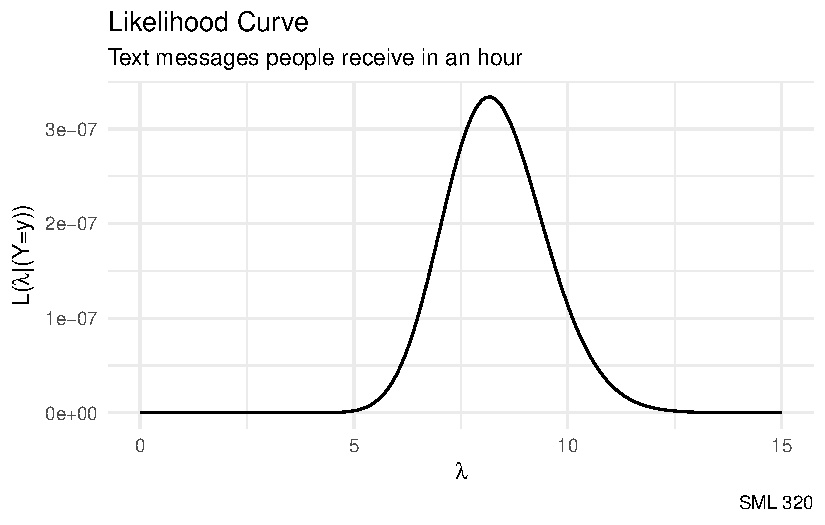
\includegraphics{ps4_code_files/figure-pdf/unnamed-chunk-1-1.pdf}

}

\end{figure}

\hypertarget{b-1}{%
\subsection{b}\label{b-1}}

\begin{Shaded}
\begin{Highlighting}[]
\NormalTok{bayesrules}\SpecialCharTok{::}\FunctionTok{plot\_gamma\_poisson}\NormalTok{(}\AttributeTok{shape =} \DecValTok{400}\NormalTok{, }\AttributeTok{rate =} \DecValTok{80}\NormalTok{,}
                               \AttributeTok{sum\_y =} \DecValTok{49}\NormalTok{, }\AttributeTok{n =} \DecValTok{6}\NormalTok{) }\SpecialCharTok{+}
  \FunctionTok{labs}\NormalTok{(}\AttributeTok{title =} \StringTok{"Gamma{-}Poisson Model"}\NormalTok{,}
       \AttributeTok{subtitle =} \StringTok{"Text Messages with Data"}\NormalTok{,}
       \AttributeTok{caption =} \StringTok{"SML 320"}\NormalTok{,}
       \AttributeTok{x =} \StringTok{"Text messages people receive in an hour"}\NormalTok{) }\SpecialCharTok{+}
  \FunctionTok{theme\_minimal}\NormalTok{() }\SpecialCharTok{+}
  \FunctionTok{theme}\NormalTok{(}\AttributeTok{legend.position =} \StringTok{"bottom"}\NormalTok{)}
\end{Highlighting}
\end{Shaded}

\begin{figure}[H]

{\centering 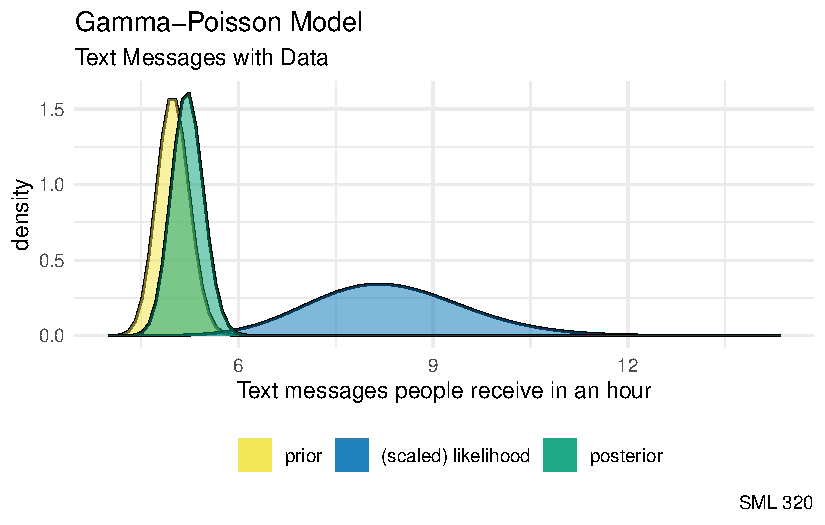
\includegraphics{ps4_code_files/figure-pdf/unnamed-chunk-2-1.pdf}

}

\end{figure}

\hypertarget{c}{%
\subsection{c}\label{c}}

\begin{Shaded}
\begin{Highlighting}[]
\NormalTok{bayesrules}\SpecialCharTok{::}\FunctionTok{summarize\_gamma\_poisson}\NormalTok{(}\AttributeTok{shape =} \DecValTok{400}\NormalTok{, }\AttributeTok{rate =} \DecValTok{80}\NormalTok{,}
                               \AttributeTok{sum\_y =} \DecValTok{49}\NormalTok{, }\AttributeTok{n =} \DecValTok{6}\NormalTok{) }\SpecialCharTok{|\textgreater{}}
  \FunctionTok{mutate\_if}\NormalTok{(is.numeric, round, }\AttributeTok{digits =} \DecValTok{4}\NormalTok{)}
\end{Highlighting}
\end{Shaded}

\begin{verbatim}
      model shape rate   mean   mode    var     sd
1     prior   400   80 5.0000 4.9875 0.0625 0.2500
2 posterior   449   86 5.2209 5.2093 0.0607 0.2464
\end{verbatim}

\hypertarget{d}{%
\subsection{d}\label{d}}

While the data from the six friends might be realistic, since we started
with an overly informative prior (i.e.~small variance), the application
of the observed data barely changed the statistics from the prior
distribution to the posterior distribution.

\hypertarget{section-2}{%
\section{5.9}\label{section-2}}

\hypertarget{a-2}{%
\subsection{a}\label{a-2}}

\begin{Shaded}
\begin{Highlighting}[]
\NormalTok{bayesrules}\SpecialCharTok{::}\FunctionTok{plot\_normal}\NormalTok{(}\AttributeTok{mean =} \FloatTok{7.2}\NormalTok{, }\AttributeTok{sd =} \FloatTok{2.6}\NormalTok{) }\SpecialCharTok{+}
  \FunctionTok{labs}\NormalTok{(}\AttributeTok{title =} \StringTok{"N(7.2, 6.76) Prior"}\NormalTok{,}
       \AttributeTok{subtitle =} \StringTok{"mean = 7.2, sd = 2.6"}\NormalTok{,}
       \AttributeTok{caption =} \StringTok{"SML 320"}\NormalTok{) }\SpecialCharTok{+}
  \FunctionTok{theme\_minimal}\NormalTok{()}
\end{Highlighting}
\end{Shaded}

\begin{figure}[H]

{\centering 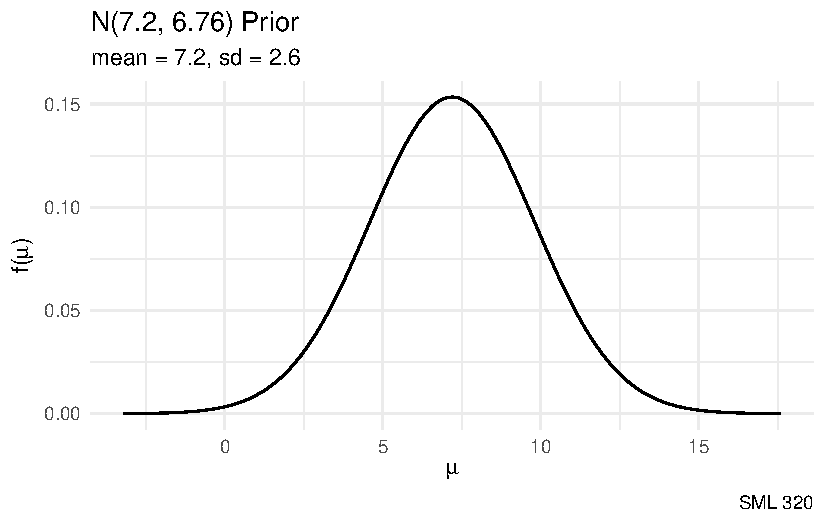
\includegraphics{ps4_code_files/figure-pdf/unnamed-chunk-4-1.pdf}

}

\end{figure}

\hypertarget{b-2}{%
\subsection{b}\label{b-2}}

\begin{Shaded}
\begin{Highlighting}[]
\FunctionTok{pnorm}\NormalTok{(}\FloatTok{7.6}\NormalTok{, }\FloatTok{7.2}\NormalTok{, }\FloatTok{2.6}\NormalTok{, }\AttributeTok{lower.tail =} \ConstantTok{FALSE}\NormalTok{)}
\end{Highlighting}
\end{Shaded}

\begin{verbatim}
[1] 0.4388655
\end{verbatim}

Yes, it seems plausible that the stock can rise by 7.6 dollars.

\hypertarget{c-1}{%
\subsection{c}\label{c-1}}

\begin{Shaded}
\begin{Highlighting}[]
\FunctionTok{pnorm}\NormalTok{(}\DecValTok{4}\NormalTok{, }\FloatTok{7.2}\NormalTok{, }\FloatTok{2.6}\NormalTok{, }\AttributeTok{lower.tail =} \ConstantTok{FALSE}\NormalTok{)}
\end{Highlighting}
\end{Shaded}

\begin{verbatim}
[1] 0.8907954
\end{verbatim}

Yes, it seems plausible that the stock can rise by 4 dollars.

\hypertarget{d-1}{%
\subsection{d}\label{d-1}}

\begin{Shaded}
\begin{Highlighting}[]
\FunctionTok{pnorm}\NormalTok{(}\DecValTok{0}\NormalTok{, }\FloatTok{7.2}\NormalTok{, }\FloatTok{2.6}\NormalTok{, }\AttributeTok{lower.tail =} \ConstantTok{TRUE}\NormalTok{)}
\end{Highlighting}
\end{Shaded}

\begin{verbatim}
[1] 0.002809441
\end{verbatim}

The prior probability of a stock price decrease is about 0.3 percent.

\hypertarget{e}{%
\subsection{e}\label{e}}

\begin{Shaded}
\begin{Highlighting}[]
\FunctionTok{pnorm}\NormalTok{(}\DecValTok{8}\NormalTok{, }\FloatTok{7.2}\NormalTok{, }\FloatTok{2.6}\NormalTok{, }\AttributeTok{lower.tail =} \ConstantTok{FALSE}\NormalTok{)}
\end{Highlighting}
\end{Shaded}

\begin{verbatim}
[1] 0.3791582
\end{verbatim}

The prior probability that the stock rises by at least 8 dollars is
about 38 percent.

\hypertarget{section-3}{%
\section{5.10}\label{section-3}}

\hypertarget{a-3}{%
\subsection{a}\label{a-3}}

\begin{Shaded}
\begin{Highlighting}[]
\NormalTok{obs\_data }\OtherTok{\textless{}{-}} \FunctionTok{c}\NormalTok{(}\SpecialCharTok{{-}}\FloatTok{0.7}\NormalTok{, }\FloatTok{1.2}\NormalTok{, }\FloatTok{4.5}\NormalTok{, }\SpecialCharTok{{-}}\DecValTok{4}\NormalTok{)}

\NormalTok{bayesrules}\SpecialCharTok{::}\FunctionTok{plot\_normal}\NormalTok{(}\AttributeTok{mean =} \FunctionTok{mean}\NormalTok{(obs\_data), }\AttributeTok{sd =} \DecValTok{2}\NormalTok{) }\SpecialCharTok{+}
  \FunctionTok{labs}\NormalTok{(}\AttributeTok{title =} \StringTok{"Normal Likelihood"}\NormalTok{,}
       \AttributeTok{subtitle =} \StringTok{"FancyStock Data"}\NormalTok{,}
       \AttributeTok{caption =} \StringTok{"SML 320"}\NormalTok{) }\SpecialCharTok{+}
  \FunctionTok{theme\_minimal}\NormalTok{()}
\end{Highlighting}
\end{Shaded}

\begin{figure}[H]

{\centering 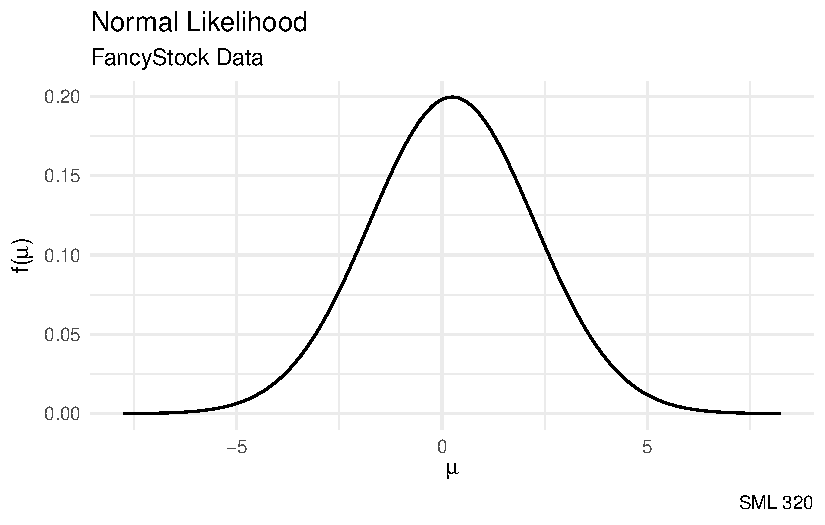
\includegraphics{ps4_code_files/figure-pdf/unnamed-chunk-9-1.pdf}

}

\end{figure}

\hypertarget{b-3}{%
\subsection{b}\label{b-3}}

\begin{Shaded}
\begin{Highlighting}[]
\NormalTok{bayesrules}\SpecialCharTok{::}\FunctionTok{plot\_normal\_normal}\NormalTok{(}
  
  \CommentTok{\# from prior}
  \AttributeTok{mean =} \FloatTok{7.6}\NormalTok{, }\AttributeTok{sd =} \FloatTok{2.6}\NormalTok{,}
  
  \CommentTok{\# from observations}
  \AttributeTok{y\_bar =} \FunctionTok{mean}\NormalTok{(obs\_data), }\AttributeTok{sigma =} \DecValTok{2}\NormalTok{, }\AttributeTok{n =} \DecValTok{4}
\NormalTok{) }\SpecialCharTok{+}
  \FunctionTok{labs}\NormalTok{(}\AttributeTok{title =} \StringTok{"Normal{-}Normal Model"}\NormalTok{,}
       \AttributeTok{subtitle =} \StringTok{"Exercise 5.5b"}\NormalTok{,}
       \AttributeTok{caption =} \StringTok{"SML 320"}\NormalTok{,}
       \AttributeTok{x =} \StringTok{"change in stock price"}\NormalTok{) }\SpecialCharTok{+}
  \FunctionTok{theme\_minimal}\NormalTok{()}
\end{Highlighting}
\end{Shaded}

\begin{figure}[H]

{\centering 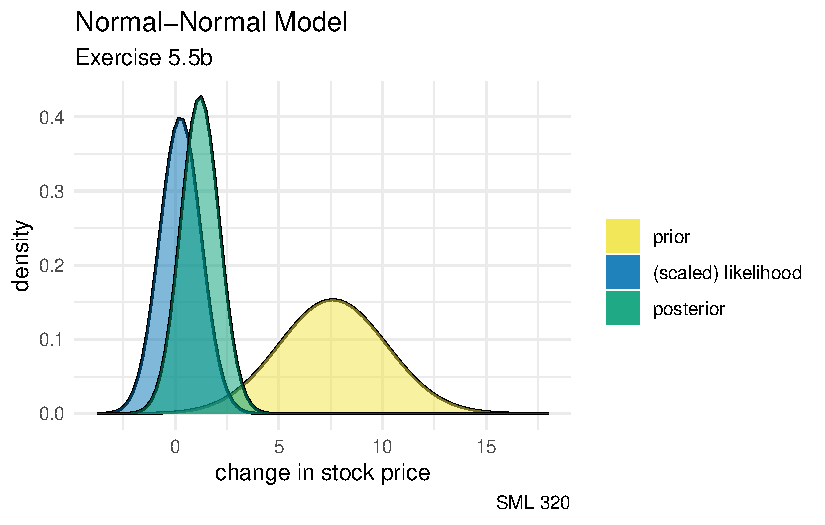
\includegraphics{ps4_code_files/figure-pdf/unnamed-chunk-10-1.pdf}

}

\end{figure}

\hypertarget{c-2}{%
\subsection{c}\label{c-2}}

\begin{Shaded}
\begin{Highlighting}[]
\NormalTok{bayesrules}\SpecialCharTok{::}\FunctionTok{summarize\_normal\_normal}\NormalTok{(}
  \CommentTok{\# from prior}
  \AttributeTok{mean =} \FloatTok{7.6}\NormalTok{, }\AttributeTok{sd =} \FloatTok{2.6}\NormalTok{,}
  
  \CommentTok{\# from observations}
  \AttributeTok{y\_bar =} \FunctionTok{mean}\NormalTok{(obs\_data), }\AttributeTok{sigma =} \DecValTok{2}\NormalTok{, }\AttributeTok{n =} \DecValTok{4}
\NormalTok{) }\SpecialCharTok{|\textgreater{}}
  \FunctionTok{mutate\_if}\NormalTok{(is.numeric, round, }\AttributeTok{digits =} \DecValTok{4}\NormalTok{)}
\end{Highlighting}
\end{Shaded}

\begin{verbatim}
      model   mean   mode    var     sd
1     prior 7.6000 7.6000 6.7600 2.6000
2 posterior 1.1972 1.1972 0.8711 0.9333
\end{verbatim}

\hypertarget{d-2}{%
\subsection{d}\label{d-2}}

Now, in the posterior distribution, the view of the stock price change
is more financially conservative with an average change of about 1.2
dollars.

\hypertarget{e-1}{%
\subsection{e}\label{e-1}}

\begin{Shaded}
\begin{Highlighting}[]
\FunctionTok{pnorm}\NormalTok{(}\DecValTok{0}\NormalTok{, }\FloatTok{1.1972}\NormalTok{, }\FloatTok{0.9333}\NormalTok{, }\AttributeTok{lower.tail =} \ConstantTok{TRUE}\NormalTok{)}
\end{Highlighting}
\end{Shaded}

\begin{verbatim}
[1] 0.09978807
\end{verbatim}

The posterior probability of a decrease in the stock price is about 10
percent.

\hypertarget{f}{%
\subsection{f}\label{f}}

\begin{Shaded}
\begin{Highlighting}[]
\FunctionTok{pnorm}\NormalTok{(}\DecValTok{8}\NormalTok{, }\FloatTok{1.1972}\NormalTok{, }\FloatTok{0.9333}\NormalTok{, }\AttributeTok{lower.tail =} \ConstantTok{FALSE}\NormalTok{)}
\end{Highlighting}
\end{Shaded}

\begin{verbatim}
[1] 1.561615e-13
\end{verbatim}

The posterior probability of the stock price increasing by over 8
dollars is virtually zero.

\hypertarget{section-4}{%
\section{6.5}\label{section-4}}

\hypertarget{a-4}{%
\subsection{a}\label{a-4}}

\begin{Shaded}
\begin{Highlighting}[]
\CommentTok{\# Step 1: Define a grid of 6 pi values}
\NormalTok{grid\_data }\OtherTok{\textless{}{-}} \FunctionTok{data.frame}\NormalTok{(}\AttributeTok{pi\_grid =} \FunctionTok{seq}\NormalTok{(}\AttributeTok{from =} \DecValTok{0}\NormalTok{, }\AttributeTok{to =} \DecValTok{1}\NormalTok{, }
                                      \AttributeTok{length =} \DecValTok{5}\NormalTok{))}

\CommentTok{\# Step 2: Evaluate the prior \& likelihood at each pi}
\NormalTok{grid\_data }\OtherTok{\textless{}{-}}\NormalTok{ grid\_data }\SpecialCharTok{\%\textgreater{}\%} 
  \FunctionTok{mutate}\NormalTok{(}\AttributeTok{prior =} \FunctionTok{dbeta}\NormalTok{(pi\_grid, }\DecValTok{3}\NormalTok{, }\DecValTok{8}\NormalTok{),}
         \AttributeTok{likelihood =} \FunctionTok{dbinom}\NormalTok{(}\DecValTok{2}\NormalTok{, }\DecValTok{10}\NormalTok{, pi\_grid))}

\CommentTok{\# Step 3: Approximate the posterior}
\NormalTok{grid\_data }\OtherTok{\textless{}{-}}\NormalTok{ grid\_data }\SpecialCharTok{\%\textgreater{}\%} 
  \FunctionTok{mutate}\NormalTok{(}\AttributeTok{unnormalized =}\NormalTok{ likelihood }\SpecialCharTok{*}\NormalTok{ prior,}
         \AttributeTok{posterior =}\NormalTok{ unnormalized }\SpecialCharTok{/} \FunctionTok{sum}\NormalTok{(unnormalized))}

\CommentTok{\# Step 4: sample from the discretized posterior}
\NormalTok{posterior\_sample }\OtherTok{\textless{}{-}} \FunctionTok{sample\_n}\NormalTok{(grid\_data, }
                             \AttributeTok{size =} \DecValTok{10000}\NormalTok{, }
                             \AttributeTok{weight =}\NormalTok{ posterior, }
                             \AttributeTok{replace =} \ConstantTok{TRUE}\NormalTok{)}

\FunctionTok{ggplot}\NormalTok{(posterior\_sample, }\FunctionTok{aes}\NormalTok{(}\AttributeTok{x =}\NormalTok{ pi\_grid)) }\SpecialCharTok{+} 
  \FunctionTok{geom\_histogram}\NormalTok{(}\FunctionTok{aes}\NormalTok{(}\AttributeTok{y =} \FunctionTok{after\_stat}\NormalTok{(density)), }
                 \AttributeTok{binwidth =} \FloatTok{0.1}\NormalTok{,}
                 \AttributeTok{fill =} \StringTok{"gray50"}\NormalTok{) }\SpecialCharTok{+} 
  \FunctionTok{stat\_function}\NormalTok{(}\AttributeTok{fun =}\NormalTok{ dbeta, }\AttributeTok{args =} \FunctionTok{list}\NormalTok{(}\DecValTok{5}\NormalTok{, }\DecValTok{16}\NormalTok{),}
                \AttributeTok{color =} \StringTok{"\#E77500"}\NormalTok{, }\AttributeTok{linewidth =} \DecValTok{3}\NormalTok{) }\SpecialCharTok{+} 
  \FunctionTok{lims}\NormalTok{(}\AttributeTok{x =} \FunctionTok{c}\NormalTok{(}\DecValTok{0}\NormalTok{, }\DecValTok{1}\NormalTok{)) }\SpecialCharTok{+}
  \FunctionTok{labs}\NormalTok{(}\AttributeTok{title =} \StringTok{"Sparse Grid: \textless{}span style=\textquotesingle{}color:\#7F7F7F\textquotesingle{}\textgreater{}simulation\textless{}/span\textgreater{} versus \textless{}span style=\textquotesingle{}color:\#E77500\textquotesingle{}\textgreater{}theoretical\textless{}/span\textgreater{}"}\NormalTok{,}
         \AttributeTok{subtitle =} \StringTok{"Beta{-}Binomial Example"}\NormalTok{,}
         \AttributeTok{caption =} \StringTok{"SML 320"}\NormalTok{) }\SpecialCharTok{+}
  \FunctionTok{theme\_minimal}\NormalTok{() }\SpecialCharTok{+}
  \FunctionTok{theme}\NormalTok{(}\AttributeTok{plot.title =} \FunctionTok{element\_markdown}\NormalTok{())}
\end{Highlighting}
\end{Shaded}

\begin{verbatim}
Warning: Removed 2 rows containing missing values (`geom_bar()`).
\end{verbatim}

\begin{figure}[H]

{\centering 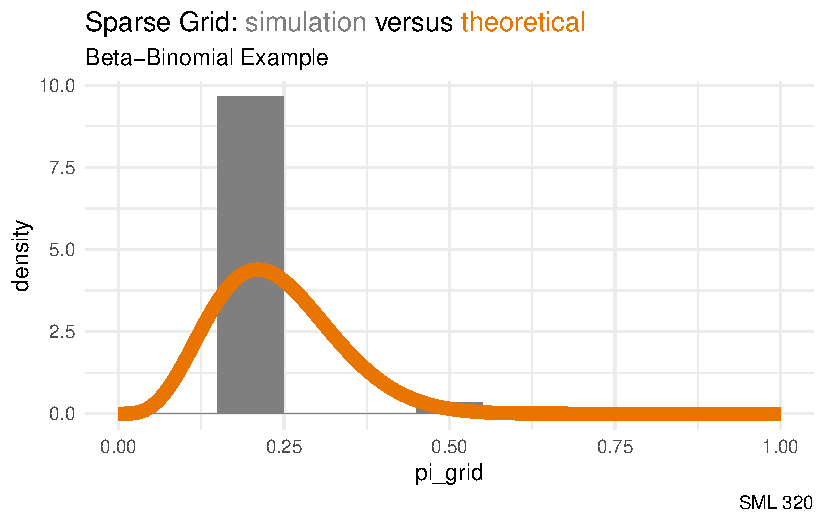
\includegraphics{ps4_code_files/figure-pdf/unnamed-chunk-14-1.pdf}

}

\end{figure}

\hypertarget{b-4}{%
\subsection{b}\label{b-4}}

\begin{Shaded}
\begin{Highlighting}[]
\CommentTok{\# Step 1: Define a grid of 6 pi values}
\NormalTok{grid\_data }\OtherTok{\textless{}{-}} \FunctionTok{data.frame}\NormalTok{(}\AttributeTok{pi\_grid =} \FunctionTok{seq}\NormalTok{(}\AttributeTok{from =} \DecValTok{0}\NormalTok{, }\AttributeTok{to =} \DecValTok{1}\NormalTok{, }
                                      \AttributeTok{length =} \DecValTok{501}\NormalTok{))}

\CommentTok{\# Step 2: Evaluate the prior \& likelihood at each pi}
\NormalTok{grid\_data }\OtherTok{\textless{}{-}}\NormalTok{ grid\_data }\SpecialCharTok{\%\textgreater{}\%} 
  \FunctionTok{mutate}\NormalTok{(}\AttributeTok{prior =} \FunctionTok{dbeta}\NormalTok{(pi\_grid, }\DecValTok{3}\NormalTok{, }\DecValTok{8}\NormalTok{),}
         \AttributeTok{likelihood =} \FunctionTok{dbinom}\NormalTok{(}\DecValTok{2}\NormalTok{, }\DecValTok{10}\NormalTok{, pi\_grid))}

\CommentTok{\# Step 3: Approximate the posterior}
\NormalTok{grid\_data }\OtherTok{\textless{}{-}}\NormalTok{ grid\_data }\SpecialCharTok{\%\textgreater{}\%} 
  \FunctionTok{mutate}\NormalTok{(}\AttributeTok{unnormalized =}\NormalTok{ likelihood }\SpecialCharTok{*}\NormalTok{ prior,}
         \AttributeTok{posterior =}\NormalTok{ unnormalized }\SpecialCharTok{/} \FunctionTok{sum}\NormalTok{(unnormalized))}

\CommentTok{\# Step 4: sample from the discretized posterior}
\NormalTok{posterior\_sample }\OtherTok{\textless{}{-}} \FunctionTok{sample\_n}\NormalTok{(grid\_data, }
                             \AttributeTok{size =} \DecValTok{10000}\NormalTok{, }
                             \AttributeTok{weight =}\NormalTok{ posterior, }
                             \AttributeTok{replace =} \ConstantTok{TRUE}\NormalTok{)}

\FunctionTok{ggplot}\NormalTok{(posterior\_sample, }\FunctionTok{aes}\NormalTok{(}\AttributeTok{x =}\NormalTok{ pi\_grid)) }\SpecialCharTok{+} 
  \FunctionTok{geom\_histogram}\NormalTok{(}\FunctionTok{aes}\NormalTok{(}\AttributeTok{y =} \FunctionTok{after\_stat}\NormalTok{(density)), }
                 \AttributeTok{binwidth =} \FloatTok{0.01}\NormalTok{,}
                 \AttributeTok{fill =} \StringTok{"gray50"}\NormalTok{) }\SpecialCharTok{+} 
  \FunctionTok{stat\_function}\NormalTok{(}\AttributeTok{fun =}\NormalTok{ dbeta, }\AttributeTok{args =} \FunctionTok{list}\NormalTok{(}\DecValTok{5}\NormalTok{, }\DecValTok{16}\NormalTok{),}
                \AttributeTok{color =} \StringTok{"\#E77500"}\NormalTok{, }\AttributeTok{linewidth =} \DecValTok{3}\NormalTok{) }\SpecialCharTok{+} 
  \FunctionTok{lims}\NormalTok{(}\AttributeTok{x =} \FunctionTok{c}\NormalTok{(}\DecValTok{0}\NormalTok{, }\DecValTok{1}\NormalTok{)) }\SpecialCharTok{+}
  \FunctionTok{labs}\NormalTok{(}\AttributeTok{title =} \StringTok{"Dense Grid: \textless{}span style=\textquotesingle{}color:\#7F7F7F\textquotesingle{}\textgreater{}simulation\textless{}/span\textgreater{} versus \textless{}span style=\textquotesingle{}color:\#E77500\textquotesingle{}\textgreater{}theoretical\textless{}/span\textgreater{}"}\NormalTok{,}
         \AttributeTok{subtitle =} \StringTok{"Beta{-}Binomial Example"}\NormalTok{,}
         \AttributeTok{caption =} \StringTok{"SML 320"}\NormalTok{) }\SpecialCharTok{+}
  \FunctionTok{theme\_minimal}\NormalTok{() }\SpecialCharTok{+}
  \FunctionTok{theme}\NormalTok{(}\AttributeTok{plot.title =} \FunctionTok{element\_markdown}\NormalTok{())}
\end{Highlighting}
\end{Shaded}

\begin{verbatim}
Warning: Removed 2 rows containing missing values (`geom_bar()`).
\end{verbatim}

\begin{figure}[H]

{\centering 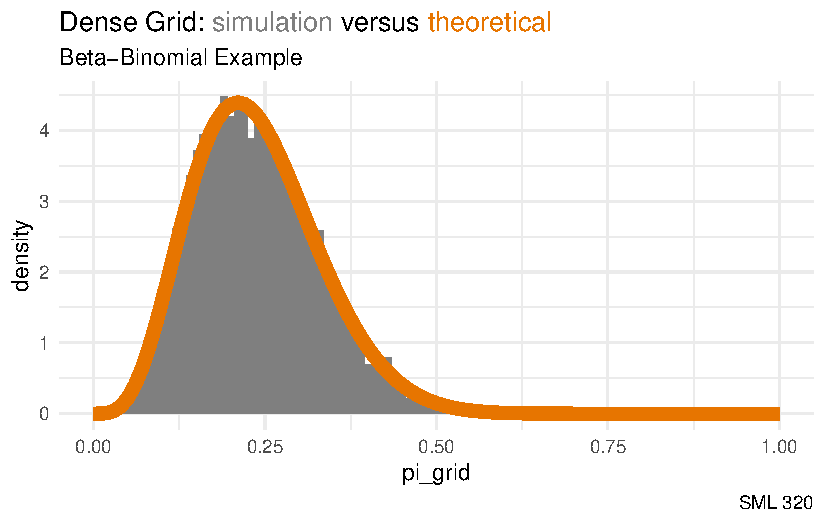
\includegraphics{ps4_code_files/figure-pdf/unnamed-chunk-15-1.pdf}

}

\end{figure}

\hypertarget{section-5}{%
\section{6.6}\label{section-5}}

\hypertarget{a-5}{%
\subsection{a}\label{a-5}}

\begin{Shaded}
\begin{Highlighting}[]
\NormalTok{obs\_counts }\OtherTok{\textless{}{-}} \FunctionTok{c}\NormalTok{(}\DecValTok{0}\NormalTok{, }\DecValTok{1}\NormalTok{, }\DecValTok{0}\NormalTok{)}

\CommentTok{\# Step 1: Define a grid of 11 pi values}
\NormalTok{grid\_data }\OtherTok{\textless{}{-}} \FunctionTok{data.frame}\NormalTok{(}\AttributeTok{lambda\_grid =} \FunctionTok{seq}\NormalTok{(}\AttributeTok{from =} \DecValTok{0}\NormalTok{, }\AttributeTok{to =} \DecValTok{8}\NormalTok{, }
                                      \AttributeTok{length =} \DecValTok{9}\NormalTok{))}

\CommentTok{\# Step 2: Evaluate the prior \& likelihood at each pi}
\NormalTok{grid\_data }\OtherTok{\textless{}{-}}\NormalTok{ grid\_data }\SpecialCharTok{\%\textgreater{}\%} 
  \FunctionTok{mutate}\NormalTok{(}\AttributeTok{prior =} \FunctionTok{dgamma}\NormalTok{(lambda\_grid, }\DecValTok{20}\NormalTok{, }\DecValTok{5}\NormalTok{),}
         \AttributeTok{likelihood =} \FunctionTok{dpois}\NormalTok{(}\DecValTok{0}\NormalTok{, lambda\_grid)}\SpecialCharTok{*}
           \FunctionTok{dpois}\NormalTok{(}\DecValTok{1}\NormalTok{, lambda\_grid)}\SpecialCharTok{*}
           \FunctionTok{dpois}\NormalTok{(}\DecValTok{0}\NormalTok{, lambda\_grid))}

\CommentTok{\# Step 3: Approximate the posterior}
\NormalTok{grid\_data }\OtherTok{\textless{}{-}}\NormalTok{ grid\_data }\SpecialCharTok{\%\textgreater{}\%} 
  \FunctionTok{mutate}\NormalTok{(}\AttributeTok{unnormalized =}\NormalTok{ likelihood }\SpecialCharTok{*}\NormalTok{ prior,}
         \AttributeTok{posterior =}\NormalTok{ unnormalized }\SpecialCharTok{/} \FunctionTok{sum}\NormalTok{(unnormalized))}

\CommentTok{\# Step 4: sample from the discretized posterior}
\NormalTok{posterior\_sample }\OtherTok{\textless{}{-}} \FunctionTok{sample\_n}\NormalTok{(grid\_data, }
                             \AttributeTok{size =} \DecValTok{10000}\NormalTok{, }
                             \AttributeTok{weight =}\NormalTok{ posterior, }
                             \AttributeTok{replace =} \ConstantTok{TRUE}\NormalTok{)}

\FunctionTok{ggplot}\NormalTok{(posterior\_sample, }\FunctionTok{aes}\NormalTok{(}\AttributeTok{x =}\NormalTok{ lambda\_grid)) }\SpecialCharTok{+} 
  \FunctionTok{geom\_histogram}\NormalTok{(}\FunctionTok{aes}\NormalTok{(}\AttributeTok{y =} \FunctionTok{after\_stat}\NormalTok{(density)), }
                 \AttributeTok{binwidth =} \FloatTok{0.5}\NormalTok{,}
                 \AttributeTok{color =} \StringTok{"black"}\NormalTok{,}
                 \AttributeTok{fill =} \StringTok{"gray50"}\NormalTok{) }\SpecialCharTok{+} 
  \FunctionTok{stat\_function}\NormalTok{(}\AttributeTok{fun =}\NormalTok{ dgamma, }\AttributeTok{args =} \FunctionTok{list}\NormalTok{(}\DecValTok{21}\NormalTok{, }\DecValTok{8}\NormalTok{),}
                \AttributeTok{color =} \StringTok{"\#E77500"}\NormalTok{, }\AttributeTok{linewidth =} \DecValTok{3}\NormalTok{) }\SpecialCharTok{+} 
  \FunctionTok{labs}\NormalTok{(}\AttributeTok{title =} \StringTok{"Sparse Grid: \textless{}span style=\textquotesingle{}color:\#7F7F7F\textquotesingle{}\textgreater{}simulation\textless{}/span\textgreater{} versus \textless{}span style=\textquotesingle{}color:\#E77500\textquotesingle{}\textgreater{}theoretical\textless{}/span\textgreater{}"}\NormalTok{,}
         \AttributeTok{subtitle =} \StringTok{"Gamma{-}Poisson Example"}\NormalTok{,}
         \AttributeTok{caption =} \StringTok{"SML 320"}\NormalTok{) }\SpecialCharTok{+}
  \FunctionTok{theme\_minimal}\NormalTok{() }\SpecialCharTok{+}
  \FunctionTok{theme}\NormalTok{(}\AttributeTok{plot.title =} \FunctionTok{element\_markdown}\NormalTok{())}
\end{Highlighting}
\end{Shaded}

\begin{figure}[H]

{\centering 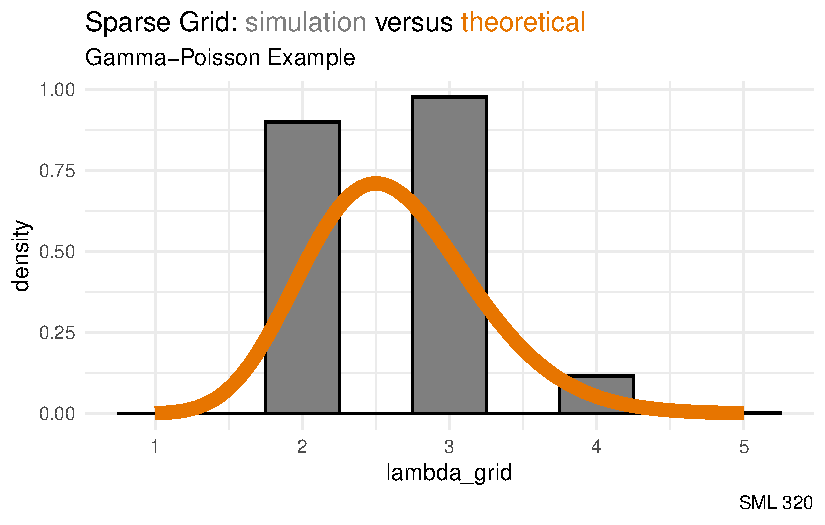
\includegraphics{ps4_code_files/figure-pdf/unnamed-chunk-16-1.pdf}

}

\end{figure}

\hypertarget{b-5}{%
\subsection{b}\label{b-5}}

\begin{Shaded}
\begin{Highlighting}[]
\NormalTok{obs\_counts }\OtherTok{\textless{}{-}} \FunctionTok{c}\NormalTok{(}\DecValTok{0}\NormalTok{, }\DecValTok{1}\NormalTok{, }\DecValTok{0}\NormalTok{)}

\CommentTok{\# Step 1: Define a grid of 11 pi values}
\NormalTok{grid\_data }\OtherTok{\textless{}{-}} \FunctionTok{data.frame}\NormalTok{(}\AttributeTok{lambda\_grid =} \FunctionTok{seq}\NormalTok{(}\AttributeTok{from =} \DecValTok{0}\NormalTok{, }\AttributeTok{to =} \DecValTok{8}\NormalTok{, }
                                      \AttributeTok{length =} \DecValTok{201}\NormalTok{))}

\CommentTok{\# Step 2: Evaluate the prior \& likelihood at each pi}
\NormalTok{grid\_data }\OtherTok{\textless{}{-}}\NormalTok{ grid\_data }\SpecialCharTok{\%\textgreater{}\%} 
  \FunctionTok{mutate}\NormalTok{(}\AttributeTok{prior =} \FunctionTok{dgamma}\NormalTok{(lambda\_grid, }\DecValTok{20}\NormalTok{, }\DecValTok{5}\NormalTok{),}
         \AttributeTok{likelihood =} \FunctionTok{dpois}\NormalTok{(}\DecValTok{0}\NormalTok{, lambda\_grid)}\SpecialCharTok{*}
           \FunctionTok{dpois}\NormalTok{(}\DecValTok{1}\NormalTok{, lambda\_grid)}\SpecialCharTok{*}
           \FunctionTok{dpois}\NormalTok{(}\DecValTok{0}\NormalTok{, lambda\_grid))}

\CommentTok{\# Step 3: Approximate the posterior}
\NormalTok{grid\_data }\OtherTok{\textless{}{-}}\NormalTok{ grid\_data }\SpecialCharTok{\%\textgreater{}\%} 
  \FunctionTok{mutate}\NormalTok{(}\AttributeTok{unnormalized =}\NormalTok{ likelihood }\SpecialCharTok{*}\NormalTok{ prior,}
         \AttributeTok{posterior =}\NormalTok{ unnormalized }\SpecialCharTok{/} \FunctionTok{sum}\NormalTok{(unnormalized))}

\CommentTok{\# Step 4: sample from the discretized posterior}
\NormalTok{posterior\_sample }\OtherTok{\textless{}{-}} \FunctionTok{sample\_n}\NormalTok{(grid\_data, }
                             \AttributeTok{size =} \DecValTok{10000}\NormalTok{, }
                             \AttributeTok{weight =}\NormalTok{ posterior, }
                             \AttributeTok{replace =} \ConstantTok{TRUE}\NormalTok{)}

\FunctionTok{ggplot}\NormalTok{(posterior\_sample, }\FunctionTok{aes}\NormalTok{(}\AttributeTok{x =}\NormalTok{ lambda\_grid)) }\SpecialCharTok{+} 
  \FunctionTok{geom\_histogram}\NormalTok{(}\FunctionTok{aes}\NormalTok{(}\AttributeTok{y =} \FunctionTok{after\_stat}\NormalTok{(density)), }
                 \AttributeTok{binwidth =} \FloatTok{0.1}\NormalTok{,}
                 \AttributeTok{color =} \StringTok{"black"}\NormalTok{,}
                 \AttributeTok{fill =} \StringTok{"gray50"}\NormalTok{) }\SpecialCharTok{+} 
  \FunctionTok{stat\_function}\NormalTok{(}\AttributeTok{fun =}\NormalTok{ dgamma, }\AttributeTok{args =} \FunctionTok{list}\NormalTok{(}\DecValTok{21}\NormalTok{, }\DecValTok{8}\NormalTok{),}
                \AttributeTok{color =} \StringTok{"\#E77500"}\NormalTok{, }\AttributeTok{linewidth =} \DecValTok{3}\NormalTok{) }\SpecialCharTok{+} 
  \FunctionTok{labs}\NormalTok{(}\AttributeTok{title =} \StringTok{"Dense Grid: \textless{}span style=\textquotesingle{}color:\#7F7F7F\textquotesingle{}\textgreater{}simulation\textless{}/span\textgreater{} versus \textless{}span style=\textquotesingle{}color:\#E77500\textquotesingle{}\textgreater{}theoretical\textless{}/span\textgreater{}"}\NormalTok{,}
         \AttributeTok{subtitle =} \StringTok{"Gamma{-}Poisson Example"}\NormalTok{,}
         \AttributeTok{caption =} \StringTok{"SML 320"}\NormalTok{) }\SpecialCharTok{+}
  \FunctionTok{theme\_minimal}\NormalTok{() }\SpecialCharTok{+}
  \FunctionTok{theme}\NormalTok{(}\AttributeTok{plot.title =} \FunctionTok{element\_markdown}\NormalTok{())}
\end{Highlighting}
\end{Shaded}

\begin{figure}[H]

{\centering 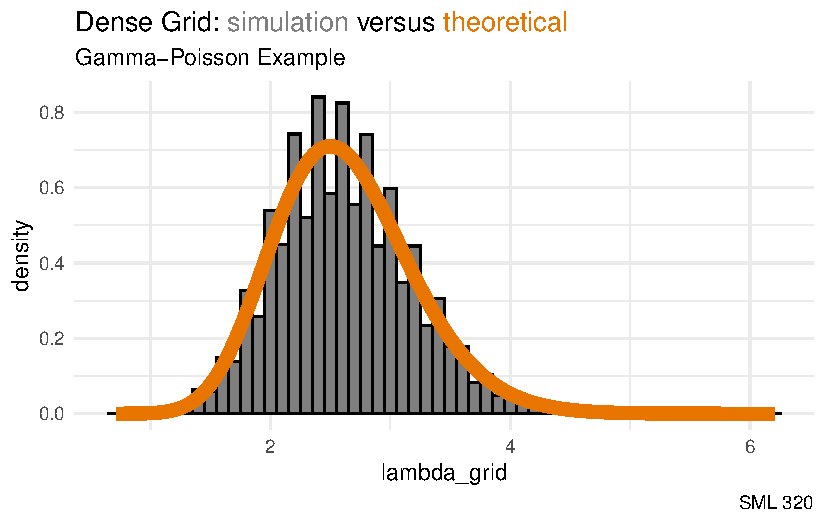
\includegraphics{ps4_code_files/figure-pdf/unnamed-chunk-17-1.pdf}

}

\end{figure}

\hypertarget{section-6}{%
\section{6.13}\label{section-6}}

\hypertarget{a-6}{%
\subsection{a}\label{a-6}}

\begin{Shaded}
\begin{Highlighting}[]
\CommentTok{\# STEP 1: DEFINE the model}
\NormalTok{bb\_model }\OtherTok{\textless{}{-}} \StringTok{"}
\StringTok{  data \{}
\StringTok{    int\textless{}lower = 0, upper = 10\textgreater{} Y;}
\StringTok{  \}}
\StringTok{  parameters \{}
\StringTok{    real\textless{}lower = 0, upper = 1\textgreater{} pi;}
\StringTok{  \}}
\StringTok{  model \{}
\StringTok{    Y \textasciitilde{} binomial(10, pi);}
\StringTok{    pi \textasciitilde{} beta(3, 8);}
\StringTok{  \}}
\StringTok{"}

\CommentTok{\# STEP 2: SIMULATE the posterior}
\NormalTok{bb\_sim }\OtherTok{\textless{}{-}} \FunctionTok{stan}\NormalTok{(}\AttributeTok{model\_code =}\NormalTok{ bb\_model, }\AttributeTok{data =} \FunctionTok{list}\NormalTok{(}\AttributeTok{Y =} \DecValTok{2}\NormalTok{), }
               \AttributeTok{chains =} \DecValTok{3}\NormalTok{, }\AttributeTok{iter =} \DecValTok{6000}\SpecialCharTok{*}\DecValTok{2}\NormalTok{, }\AttributeTok{seed =} \DecValTok{84735}\NormalTok{)}
\end{Highlighting}
\end{Shaded}

\begin{verbatim}

SAMPLING FOR MODEL 'anon_model' NOW (CHAIN 1).
Chain 1: 
Chain 1: Gradient evaluation took 1.1e-05 seconds
Chain 1: 1000 transitions using 10 leapfrog steps per transition would take 0.11 seconds.
Chain 1: Adjust your expectations accordingly!
Chain 1: 
Chain 1: 
Chain 1: Iteration:     1 / 12000 [  0%]  (Warmup)
Chain 1: Iteration:  1200 / 12000 [ 10%]  (Warmup)
Chain 1: Iteration:  2400 / 12000 [ 20%]  (Warmup)
Chain 1: Iteration:  3600 / 12000 [ 30%]  (Warmup)
Chain 1: Iteration:  4800 / 12000 [ 40%]  (Warmup)
Chain 1: Iteration:  6000 / 12000 [ 50%]  (Warmup)
Chain 1: Iteration:  6001 / 12000 [ 50%]  (Sampling)
Chain 1: Iteration:  7200 / 12000 [ 60%]  (Sampling)
Chain 1: Iteration:  8400 / 12000 [ 70%]  (Sampling)
Chain 1: Iteration:  9600 / 12000 [ 80%]  (Sampling)
Chain 1: Iteration: 10800 / 12000 [ 90%]  (Sampling)
Chain 1: Iteration: 12000 / 12000 [100%]  (Sampling)
Chain 1: 
Chain 1:  Elapsed Time: 0.038 seconds (Warm-up)
Chain 1:                0.034 seconds (Sampling)
Chain 1:                0.072 seconds (Total)
Chain 1: 

SAMPLING FOR MODEL 'anon_model' NOW (CHAIN 2).
Chain 2: 
Chain 2: Gradient evaluation took 2e-06 seconds
Chain 2: 1000 transitions using 10 leapfrog steps per transition would take 0.02 seconds.
Chain 2: Adjust your expectations accordingly!
Chain 2: 
Chain 2: 
Chain 2: Iteration:     1 / 12000 [  0%]  (Warmup)
Chain 2: Iteration:  1200 / 12000 [ 10%]  (Warmup)
Chain 2: Iteration:  2400 / 12000 [ 20%]  (Warmup)
Chain 2: Iteration:  3600 / 12000 [ 30%]  (Warmup)
Chain 2: Iteration:  4800 / 12000 [ 40%]  (Warmup)
Chain 2: Iteration:  6000 / 12000 [ 50%]  (Warmup)
Chain 2: Iteration:  6001 / 12000 [ 50%]  (Sampling)
Chain 2: Iteration:  7200 / 12000 [ 60%]  (Sampling)
Chain 2: Iteration:  8400 / 12000 [ 70%]  (Sampling)
Chain 2: Iteration:  9600 / 12000 [ 80%]  (Sampling)
Chain 2: Iteration: 10800 / 12000 [ 90%]  (Sampling)
Chain 2: Iteration: 12000 / 12000 [100%]  (Sampling)
Chain 2: 
Chain 2:  Elapsed Time: 0.034 seconds (Warm-up)
Chain 2:                0.035 seconds (Sampling)
Chain 2:                0.069 seconds (Total)
Chain 2: 

SAMPLING FOR MODEL 'anon_model' NOW (CHAIN 3).
Chain 3: 
Chain 3: Gradient evaluation took 1e-06 seconds
Chain 3: 1000 transitions using 10 leapfrog steps per transition would take 0.01 seconds.
Chain 3: Adjust your expectations accordingly!
Chain 3: 
Chain 3: 
Chain 3: Iteration:     1 / 12000 [  0%]  (Warmup)
Chain 3: Iteration:  1200 / 12000 [ 10%]  (Warmup)
Chain 3: Iteration:  2400 / 12000 [ 20%]  (Warmup)
Chain 3: Iteration:  3600 / 12000 [ 30%]  (Warmup)
Chain 3: Iteration:  4800 / 12000 [ 40%]  (Warmup)
Chain 3: Iteration:  6000 / 12000 [ 50%]  (Warmup)
Chain 3: Iteration:  6001 / 12000 [ 50%]  (Sampling)
Chain 3: Iteration:  7200 / 12000 [ 60%]  (Sampling)
Chain 3: Iteration:  8400 / 12000 [ 70%]  (Sampling)
Chain 3: Iteration:  9600 / 12000 [ 80%]  (Sampling)
Chain 3: Iteration: 10800 / 12000 [ 90%]  (Sampling)
Chain 3: Iteration: 12000 / 12000 [100%]  (Sampling)
Chain 3: 
Chain 3:  Elapsed Time: 0.034 seconds (Warm-up)
Chain 3:                0.035 seconds (Sampling)
Chain 3:                0.069 seconds (Total)
Chain 3: 
\end{verbatim}

\hypertarget{b-6}{%
\subsection{b}\label{b-6}}

\begin{Shaded}
\begin{Highlighting}[]
\NormalTok{bayesplot}\SpecialCharTok{::}\FunctionTok{mcmc\_trace}\NormalTok{(bb\_sim, }\AttributeTok{pars =} \StringTok{"pi"}\NormalTok{, }\AttributeTok{size =} \FloatTok{0.1}\NormalTok{)}
\end{Highlighting}
\end{Shaded}

\begin{figure}[H]

{\centering 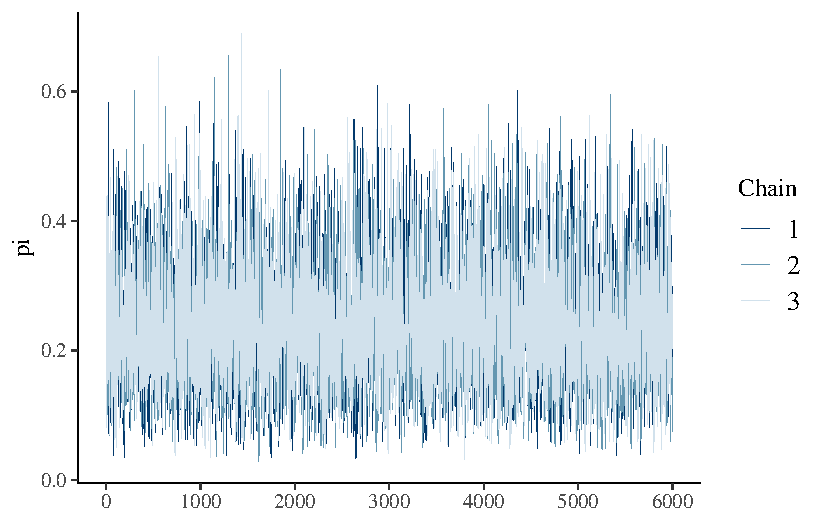
\includegraphics{ps4_code_files/figure-pdf/unnamed-chunk-19-1.pdf}

}

\end{figure}

\hypertarget{c-3}{%
\subsection{c}\label{c-3}}

The trace plot displays only the last 6000 elements of each chain
because we are disregarding the ``burn-in'' start of the MCMC.

\hypertarget{d-3}{%
\subsection{d}\label{d-3}}

\begin{Shaded}
\begin{Highlighting}[]
\NormalTok{bayesplot}\SpecialCharTok{::}\FunctionTok{mcmc\_dens}\NormalTok{(bb\_sim, }\AttributeTok{pars =} \StringTok{"pi"}\NormalTok{) }\SpecialCharTok{+} 
  \FunctionTok{stat\_function}\NormalTok{(}\AttributeTok{fun =}\NormalTok{ dbeta, }\AttributeTok{args =} \FunctionTok{list}\NormalTok{(}\DecValTok{5}\NormalTok{, }\DecValTok{16}\NormalTok{),}
                \AttributeTok{color =} \StringTok{"\#E77500"}\NormalTok{, }\AttributeTok{linewidth =} \DecValTok{3}\NormalTok{) }\SpecialCharTok{+} 
  \FunctionTok{labs}\NormalTok{(}\AttributeTok{title =} \StringTok{"MCMC: \textless{}span style=\textquotesingle{}color:\#619CFF\textquotesingle{}\textgreater{}simulation\textless{}/span\textgreater{} versus \textless{}span style=\textquotesingle{}color:\#E77500\textquotesingle{}\textgreater{}theoretical\textless{}/span\textgreater{}"}\NormalTok{,}
         \AttributeTok{subtitle =} \StringTok{"Beta{-}Binomial Example"}\NormalTok{,}
         \AttributeTok{caption =} \StringTok{"SML 320"}\NormalTok{) }\SpecialCharTok{+}
  \FunctionTok{theme\_minimal}\NormalTok{() }\SpecialCharTok{+}
  \FunctionTok{theme}\NormalTok{(}\AttributeTok{plot.title =} \FunctionTok{element\_markdown}\NormalTok{())}
\end{Highlighting}
\end{Shaded}

\begin{figure}[H]

{\centering 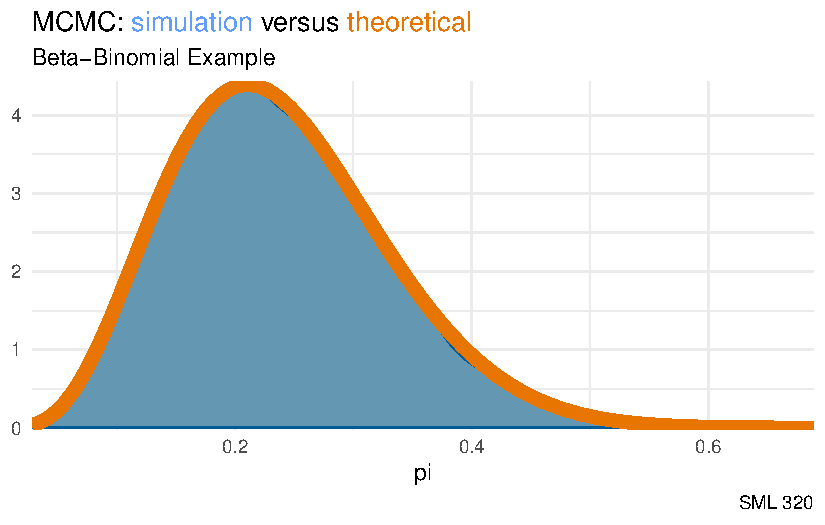
\includegraphics{ps4_code_files/figure-pdf/unnamed-chunk-20-1.pdf}

}

\end{figure}

\hypertarget{e-2}{%
\subsection{e}\label{e-2}}

The simulation seems to align with the Beta(5,16) posterior model that
we expect.

\hypertarget{section-7}{%
\section{6.15}\label{section-7}}

\hypertarget{a-7}{%
\subsection{a}\label{a-7}}

\begin{Shaded}
\begin{Highlighting}[]
\CommentTok{\# STEP 1: DEFINE the model}
\NormalTok{gp\_model }\OtherTok{\textless{}{-}} \StringTok{"}
\StringTok{  data \{}
\StringTok{    int\textless{}lower = 0\textgreater{} Y[3];}
\StringTok{  \}}
\StringTok{  parameters \{}
\StringTok{    real\textless{}lower = 0\textgreater{} lambda;}
\StringTok{  \}}
\StringTok{  model \{}
\StringTok{    Y \textasciitilde{} poisson(lambda);}
\StringTok{    lambda \textasciitilde{} gamma(20, 5);}
\StringTok{  \}}
\StringTok{"}

\CommentTok{\# STEP 2: SIMULATE the posterior}
\NormalTok{obs\_counts }\OtherTok{\textless{}{-}} \FunctionTok{c}\NormalTok{(}\DecValTok{0}\NormalTok{, }\DecValTok{1}\NormalTok{, }\DecValTok{0}\NormalTok{)}
\NormalTok{gp\_sim }\OtherTok{\textless{}{-}} \FunctionTok{stan}\NormalTok{(}\AttributeTok{model\_code =}\NormalTok{ gp\_model, }
               \AttributeTok{data =} \FunctionTok{list}\NormalTok{(}\AttributeTok{Y =}\NormalTok{ obs\_counts), }
               \AttributeTok{chains =} \DecValTok{4}\NormalTok{, }\AttributeTok{iter =} \DecValTok{5000}\SpecialCharTok{*}\DecValTok{2}\NormalTok{, }\AttributeTok{seed =} \DecValTok{84735}\NormalTok{)}
\end{Highlighting}
\end{Shaded}

\begin{verbatim}

SAMPLING FOR MODEL 'anon_model' NOW (CHAIN 1).
Chain 1: 
Chain 1: Gradient evaluation took 1.7e-05 seconds
Chain 1: 1000 transitions using 10 leapfrog steps per transition would take 0.17 seconds.
Chain 1: Adjust your expectations accordingly!
Chain 1: 
Chain 1: 
Chain 1: Iteration:    1 / 10000 [  0%]  (Warmup)
Chain 1: Iteration: 1000 / 10000 [ 10%]  (Warmup)
Chain 1: Iteration: 2000 / 10000 [ 20%]  (Warmup)
Chain 1: Iteration: 3000 / 10000 [ 30%]  (Warmup)
Chain 1: Iteration: 4000 / 10000 [ 40%]  (Warmup)
Chain 1: Iteration: 5000 / 10000 [ 50%]  (Warmup)
Chain 1: Iteration: 5001 / 10000 [ 50%]  (Sampling)
Chain 1: Iteration: 6000 / 10000 [ 60%]  (Sampling)
Chain 1: Iteration: 7000 / 10000 [ 70%]  (Sampling)
Chain 1: Iteration: 8000 / 10000 [ 80%]  (Sampling)
Chain 1: Iteration: 9000 / 10000 [ 90%]  (Sampling)
Chain 1: Iteration: 10000 / 10000 [100%]  (Sampling)
Chain 1: 
Chain 1:  Elapsed Time: 0.031 seconds (Warm-up)
Chain 1:                0.031 seconds (Sampling)
Chain 1:                0.062 seconds (Total)
Chain 1: 

SAMPLING FOR MODEL 'anon_model' NOW (CHAIN 2).
Chain 2: 
Chain 2: Gradient evaluation took 3e-06 seconds
Chain 2: 1000 transitions using 10 leapfrog steps per transition would take 0.03 seconds.
Chain 2: Adjust your expectations accordingly!
Chain 2: 
Chain 2: 
Chain 2: Iteration:    1 / 10000 [  0%]  (Warmup)
Chain 2: Iteration: 1000 / 10000 [ 10%]  (Warmup)
Chain 2: Iteration: 2000 / 10000 [ 20%]  (Warmup)
Chain 2: Iteration: 3000 / 10000 [ 30%]  (Warmup)
Chain 2: Iteration: 4000 / 10000 [ 40%]  (Warmup)
Chain 2: Iteration: 5000 / 10000 [ 50%]  (Warmup)
Chain 2: Iteration: 5001 / 10000 [ 50%]  (Sampling)
Chain 2: Iteration: 6000 / 10000 [ 60%]  (Sampling)
Chain 2: Iteration: 7000 / 10000 [ 70%]  (Sampling)
Chain 2: Iteration: 8000 / 10000 [ 80%]  (Sampling)
Chain 2: Iteration: 9000 / 10000 [ 90%]  (Sampling)
Chain 2: Iteration: 10000 / 10000 [100%]  (Sampling)
Chain 2: 
Chain 2:  Elapsed Time: 0.031 seconds (Warm-up)
Chain 2:                0.029 seconds (Sampling)
Chain 2:                0.06 seconds (Total)
Chain 2: 

SAMPLING FOR MODEL 'anon_model' NOW (CHAIN 3).
Chain 3: 
Chain 3: Gradient evaluation took 3e-06 seconds
Chain 3: 1000 transitions using 10 leapfrog steps per transition would take 0.03 seconds.
Chain 3: Adjust your expectations accordingly!
Chain 3: 
Chain 3: 
Chain 3: Iteration:    1 / 10000 [  0%]  (Warmup)
Chain 3: Iteration: 1000 / 10000 [ 10%]  (Warmup)
Chain 3: Iteration: 2000 / 10000 [ 20%]  (Warmup)
Chain 3: Iteration: 3000 / 10000 [ 30%]  (Warmup)
Chain 3: Iteration: 4000 / 10000 [ 40%]  (Warmup)
Chain 3: Iteration: 5000 / 10000 [ 50%]  (Warmup)
Chain 3: Iteration: 5001 / 10000 [ 50%]  (Sampling)
Chain 3: Iteration: 6000 / 10000 [ 60%]  (Sampling)
Chain 3: Iteration: 7000 / 10000 [ 70%]  (Sampling)
Chain 3: Iteration: 8000 / 10000 [ 80%]  (Sampling)
Chain 3: Iteration: 9000 / 10000 [ 90%]  (Sampling)
Chain 3: Iteration: 10000 / 10000 [100%]  (Sampling)
Chain 3: 
Chain 3:  Elapsed Time: 0.035 seconds (Warm-up)
Chain 3:                0.032 seconds (Sampling)
Chain 3:                0.067 seconds (Total)
Chain 3: 

SAMPLING FOR MODEL 'anon_model' NOW (CHAIN 4).
Chain 4: 
Chain 4: Gradient evaluation took 2e-06 seconds
Chain 4: 1000 transitions using 10 leapfrog steps per transition would take 0.02 seconds.
Chain 4: Adjust your expectations accordingly!
Chain 4: 
Chain 4: 
Chain 4: Iteration:    1 / 10000 [  0%]  (Warmup)
Chain 4: Iteration: 1000 / 10000 [ 10%]  (Warmup)
Chain 4: Iteration: 2000 / 10000 [ 20%]  (Warmup)
Chain 4: Iteration: 3000 / 10000 [ 30%]  (Warmup)
Chain 4: Iteration: 4000 / 10000 [ 40%]  (Warmup)
Chain 4: Iteration: 5000 / 10000 [ 50%]  (Warmup)
Chain 4: Iteration: 5001 / 10000 [ 50%]  (Sampling)
Chain 4: Iteration: 6000 / 10000 [ 60%]  (Sampling)
Chain 4: Iteration: 7000 / 10000 [ 70%]  (Sampling)
Chain 4: Iteration: 8000 / 10000 [ 80%]  (Sampling)
Chain 4: Iteration: 9000 / 10000 [ 90%]  (Sampling)
Chain 4: Iteration: 10000 / 10000 [100%]  (Sampling)
Chain 4: 
Chain 4:  Elapsed Time: 0.031 seconds (Warm-up)
Chain 4:                0.033 seconds (Sampling)
Chain 4:                0.064 seconds (Total)
Chain 4: 
\end{verbatim}

\hypertarget{b-7}{%
\subsection{b}\label{b-7}}

\begin{Shaded}
\begin{Highlighting}[]
\NormalTok{bayesplot}\SpecialCharTok{::}\FunctionTok{mcmc\_trace}\NormalTok{(gp\_sim, }\AttributeTok{pars =} \StringTok{"lambda"}\NormalTok{, }\AttributeTok{size =} \FloatTok{0.1}\NormalTok{)}
\end{Highlighting}
\end{Shaded}

\begin{figure}[H]

{\centering 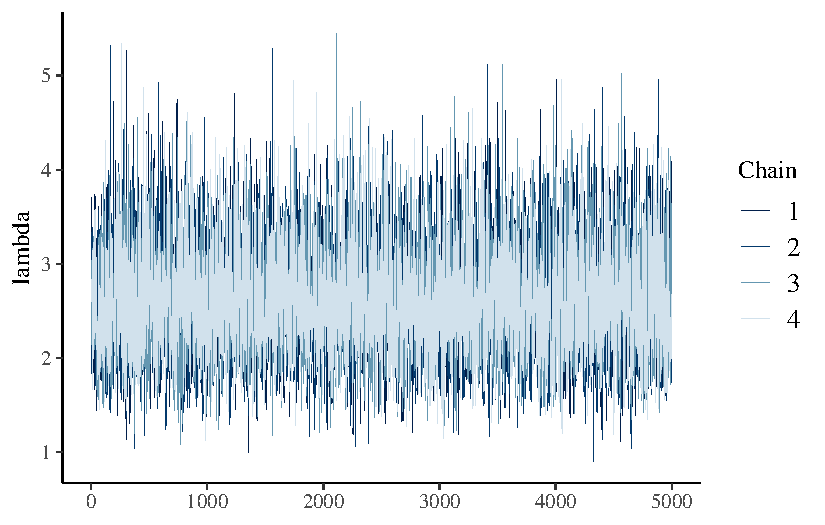
\includegraphics{ps4_code_files/figure-pdf/unnamed-chunk-22-1.pdf}

}

\end{figure}

\begin{Shaded}
\begin{Highlighting}[]
\NormalTok{bayesplot}\SpecialCharTok{::}\FunctionTok{mcmc\_dens}\NormalTok{(gp\_sim, }\AttributeTok{pars =} \StringTok{"lambda"}\NormalTok{) }\SpecialCharTok{+} 
  \FunctionTok{stat\_function}\NormalTok{(}\AttributeTok{fun =}\NormalTok{ dgamma, }\AttributeTok{args =} \FunctionTok{list}\NormalTok{(}\DecValTok{21}\NormalTok{, }\DecValTok{8}\NormalTok{),}
                \AttributeTok{color =} \StringTok{"\#E77500"}\NormalTok{, }\AttributeTok{linewidth =} \DecValTok{3}\NormalTok{) }\SpecialCharTok{+} 
  \FunctionTok{labs}\NormalTok{(}\AttributeTok{title =} \StringTok{"MCMC: \textless{}span style=\textquotesingle{}color:\#619CFF\textquotesingle{}\textgreater{}simulation\textless{}/span\textgreater{} versus \textless{}span style=\textquotesingle{}color:\#E77500\textquotesingle{}\textgreater{}theoretical\textless{}/span\textgreater{}"}\NormalTok{,}
         \AttributeTok{subtitle =} \StringTok{"Gamma{-}Poisson Example"}\NormalTok{,}
         \AttributeTok{caption =} \StringTok{"SML 320"}\NormalTok{) }\SpecialCharTok{+}
  \FunctionTok{theme\_minimal}\NormalTok{() }\SpecialCharTok{+}
  \FunctionTok{theme}\NormalTok{(}\AttributeTok{plot.title =} \FunctionTok{element\_markdown}\NormalTok{())}
\end{Highlighting}
\end{Shaded}

\begin{figure}[H]

{\centering 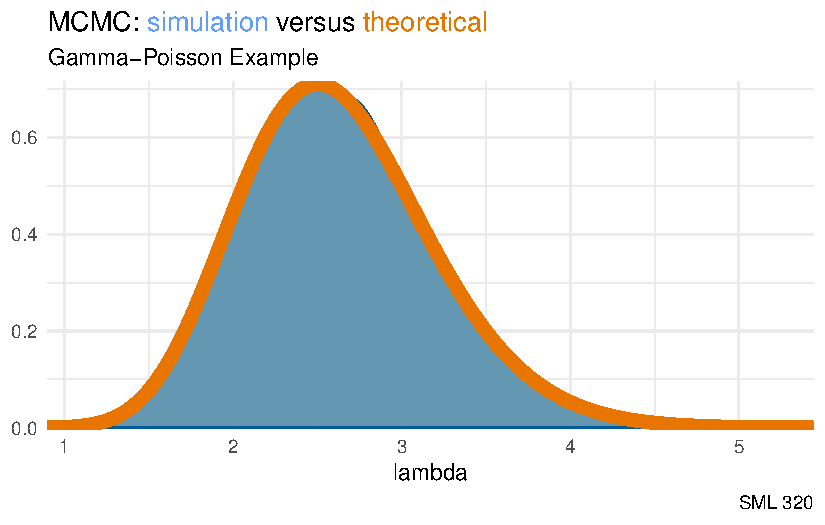
\includegraphics{ps4_code_files/figure-pdf/unnamed-chunk-23-1.pdf}

}

\end{figure}

\hypertarget{c-4}{%
\subsection{c}\label{c-4}}

From our density plots, the mode from the MCMC seems to be about 2.5

\hypertarget{section-8}{%
\subsection{}\label{section-8}}

The simulation seems to align with the Gamma(21,8) posterior model that
we expect.



\end{document}
